\chapter{Contribuição}
\label{cap_contribuicao}

Nesta secção, será relatado o trabalho realizado no intuito da componente prática do projeto e os resultados. 
% Neste caso, relevante à criação de um \textit{toolkit} e ferramentas para a extração do conteúdo de documentos antigos, em particular jornais, com melhores resultados do que os oferecidos pelas ferramentas de \acrshort{ocr} base e, possibilitando a obtenção da lógica e organização original dos mesmos.

\section{Introdução}
% Ao longo do período de inicialização da dissertação: desde a definição dos objetivos do projeto, aprofundamento da temática e estudo do estado da arte; de forma a simultaneamente acostumar com as tecnologias, assim como ganhar um melhor entendimento sobre os algoritmos a implementar e os desafios apresentados, algum trabalho prático já foi realizado. 
% Este envolve principalmente a criação de uma ferramenta para facilitar a visualização dos resultados de reconhecimento, assim como o debugging destes e alguns algoritmos preliminares para manipulação destes resultados de \acrshort{ocr}.

A discussão sobre o trabalho realizado será estruturada em 3 componentes principais.
\begin{itemize}
	\item Ferramentas do \textit{toolkit} desenvolvidas
	\item Pipeline de aplicação do toolkit
% 	\item GUI de aplicação geral do \textit{toolkit}
	\item GUI editor OCR
\end{itemize}

Para cada uma das secções delimitadas, será dada uma explicação do seu propósito e produto sumariado, procedido por uma discussão mais detalhada dos elementos que a constituem.

De forma geral, o código desenvolvido foi maioritariamente escrito em Python, com algumas instâncias de C.

\section{Ferramentas do \textit{toolkit} desenvolvidas}

\subsection{Introdução}

A componente do \textit{toolkit} foi a premissa base do tema da dissertação. Um conjunto de ferramentas focado na melhoria dos resultados obtidos da aplicação de \acrshort{ocr} em documentos antigos, com especial interesse em jornais. 

Estas ferramentas são então pertinentes para os diversos passos do processo convencional de \acrshort{ocr}, i.e. pré-processamento, OCR e pós-processamento; atendendo tanto a processamento de imagem, processamento de resultados de OCR e texto, e validação de resultados.

Além dos métodos principais criados para a resolução de problemas identificados, é importante realçar certos pontos essenciais que serviram como base para o resto do trabalho. Estes são as estruturas de dados utilizadas para o tratamento dos resultados de OCR.

\subsection{Sumário}

\begin{itemize}\setlength\itemsep{0.05cm}
	\item Estruturas de dados \ref{data_structures}
	\begin{itemize}\setlength\itemsep{0.05cm}
		\item OCR Tree \ref{ocr_tree}
		\item Box
	\end{itemize}
	\item Métodos
	
	\begin{itemize}\setlength\itemsep{0.05cm}
		\item Processamento de resultados OCR
		
		\begin{itemize}\setlength\itemsep{0.05cm}
			\item Conversão de resultados OCR
			\item Análise de texto
			\item Limpeza de OCR Tree
			\item Categorização de Blocos
			\item Divisão de blocos
			\item Cálculo de ordem de leitura
			\item Segmentação de resultados 
		\end{itemize}
		
		\item Processamento de imagem
		\begin{itemize}\setlength\itemsep{0.05cm}
			\item Binarização de imagem
			\item Rotação de imagem
			\item Cálculo de sentido de rotação
			\item Segmentação de documento
			\item Identificação de imagens
			\item Identificação de delimitadores
			\item Divisão de colunas 
		\end{itemize}
		
		\item Processamento de texto
		\begin{itemize}\setlength\itemsep{0.05cm}
			\item Limpeza de hifenização
		\end{itemize}
		
	\end{itemize}
	
\end{itemize}


\subsection{Estruturas de dados}
\label{data_structures}


\subsubsection{OCR Tree}
\label{ocr_tree}

Como o produto final do projeto intende aceitar diferentes tipos de resultados OCR, i.e. resultantes de diferentes motores OCR ou de ficheiros como hOCR que já possuem os resultados, existe uma necessidade de converter estes diferentes formatos num único tipo que mantenha a informação base pretendida.

Estruturas de dados standard como \citep{hocr_doc} ou \citep{alto_doc} apresentam um resultado final semelhante e com capacidade base de armazenamento de meta-dados superior porém, sendo baseados em XML, tornam a sua manipulação mais complexa e, em múltiplos casos a informação proporcionada é além do necessário ou gera conclusões erradas quando gerado de output automático (ex.: atribuição de classes caption a blocos que são títulos). Assim sendo, embora tenha sido desenvolvido um conversor de, e para HOCR, para o atual projeto optou-se pela criação de uma estrutura de dados própria.

Deste modo, tomando como inspiração os atributos dos resultados do Tesseract no modo de dicionário \citep{tesseract_doc}, foi implementada uma estrutura de dados no formato de árvore de dados.

A escolha de uma estrutura de árvore permite a hierarquização de blocos de acordo com o seu nível, quer exista uma divisão de nível à partida, como é o caso do Tesseract que segue: página $\longrightarrow$ bloco $\longrightarrow$ parágrafo $\longrightarrow$ linha $\longrightarrow$ palavra; ou apenas um único nível, semelhante ao Keras-OCR.

Todos os algoritmos desenvolvidos, inclusive os métodos para visualização (métodos de debugging e GUI desenvolvido), assumem e trabalham com os dados de OCR no formato desta estrutura de dados.

As características mais relevantes desta estrutura são:

\begin{itemize}\setlength\itemsep{0.05cm}
	\item \textbf{Level} : Nível/altura do nodo.
	\begin{itemize}\setlength\itemsep{0.05cm}
		\item documento : 0
		\item página 	: 1
		\item bloco		: 2
		\item parágrafo : 3
		\item linha 	: 4
		\item palavra	: 5
	\end{itemize}\setlength\itemsep{0.05cm}
	\item \textbf{(page|block|par|line|word)\_num}: Identificação da ordem (dentro de outras caixas(ex.: linha), se aplicável)
	\item \textbf{text} : Texto do bloco, normalmente apenas preenchido ao nível da palavra
	\item \textbf{conf} : Confiança no texto
	\item \textbf{id}
	\item \textbf{type} : Tipo do bloco, ex.: delimitador, título
	\item \textbf{children}
	\item \textbf{box}: Bounding box do nodo, representado pela estrutura de dados Box, que também possui métodos para transformações e verificações geométricas ou de características.
	\item Características de texto: ex.: texto iniciado (start\_text); texto não terminado (end\_text).
\end{itemize}

Construtores da classe são capazes de admitir outros atributos não base de modo a expandir a utilidade da estrutura. Construtores disponíveis: iniciação por argumentos, dicionário, ficheiro JSON e ficheiro HOCR.

Da mesma forma, conversores para estes ficheiros compreendidos para iniciação também foram desenvolvidos.

A classe possuí por métodos de transformação e análise sobre a árvore OCR que facilitam a manipulação dos resultados OCR. 

Alguns dos métodos mais relevantes definidos são:

\begin{itemize}\setlength\itemsep{0.05cm}
	\item \textbf{id\_boxes} : Adiciona identificador aos blocos.
	
	Argumentos:
		\begin{itemize}\setlength\itemsep{0.05cm}
			\item level : lista de níveis onde adicionar identificador
			\item ids (opt): dicionário de ids a utilizar caso não se queira iniciar no 0.
			\item delimiters (opt): flag para identificar delimitadores
			\item area (opt): argumento do tipo Box, que restringe os nodos a identificar a uma dada área
			\item override (opt): flag para reescrever id se já existe.
		\end{itemize}
				
	\item \textbf{calculate\_mean\_height} : Calcula a altura média das caixas de um dado nível.
	
	Argumentos:
	\begin{itemize}\setlength\itemsep{0.05cm}
		\item level : nível a calcular
		\item conf (opt): valor de confiança de texto no caso de apenas serem relevantes caixas com certa confiança (aplicável apenas para nível de texto)
	\end{itemize}
	
	
	\item \textbf{is\_text\_size} : Verifica se um nodo se encontra dentro do tamanho de texto.
	
	Argumentos:
	\begin{itemize}\setlength\itemsep{0.05cm}
		\item text\_size : tamanho de texto a comparar
		\item mean\_height (opt): altura do bloco, caso já tenha sido calculado
		\item range : margem de erro aceitável (relativo)
		\item level : nível das caixas usado caso seja necessário calcular a altura média
		\item conf : confiança do texto a utilizar para calcular a altura média
	\end{itemize}
	
	\item \textbf{is\_empty} : Verifica se um nodo é vazio.
	
	Argumentos:
	\begin{itemize}\setlength\itemsep{0.05cm}
		\item conf : confiança de texto a utilizar para considerar palavras válidas
		\item only\_text : flag que dita se o tipo do bloco influencia o resultado, i.e. blocos de tipo "image" não são vazios
	\end{itemize}
	
	
	\item \textbf{text\_is\_title} : Verifica se um nodo é potencial título.
	
	Algoritmo: Caixa não é texto vertical e é maior do que o tamanho normal de texto.
	
	
	Argumentos:
	\begin{itemize}\setlength\itemsep{0.05cm}
		\item normal\_text\_size : tamanho de texto considerado como normal
		\item conf : confiança de texto a utilizar para considerar palavras válidas
		\item range : margem de acerto aceitável (relativo)
		\item level : nível usado para calcular o tamanho médio do bloco
	\end{itemize}
	
	
	\item \textbf{is\_delimiter} : Verifica se um nodo é potencial delimitador.
	
	Algoritmo: Caixa já é do tipo delimitador, ou é vazia e $ box.width >= box.height*4 || box.height >= box.widht*4 $.
	
	
	Argumentos:
	\begin{itemize}\setlength\itemsep{0.05cm}
		\item conf : confiança de texto a utilizar para considerar palavras válidas
		\item only\_type : flag que dita se usa apenas o tipo do nodo para a verificação
	\end{itemize}
	
	
	\item \textbf{is\_image} : Verifica se um nodo é potencial imagem.
	
	Algoritmo: Caixa já é do tipo imagem ou, é vazia, não é um delimitador e é 3 vezes mais alta do que o tamanho de texto.
	
	
	Argumentos:
	\begin{itemize}\setlength\itemsep{0.05cm}
		\item conf : confiança de texto a utilizar para considerar palavras válidas
		\item text\_size : tamanho de texto a utilizar para comparação com altura da caixa
		\item only\_type : flag que dita se usa apenas o tipo do nodo para a verificação
	\end{itemize}
	
	
	\item \textbf{is\_vertical\_text} : Verifica se um nodo é texto vertical.
	
	Algoritmo: 
	
	\begin{algorithm}[H]
		\caption{Verificação de texto vertical}
		\algsetup{linenosize=\tiny}
		\scriptsize
		\begin{algorithmic}[1]
			\IF{nodo não é vazio}
				\STATE lines
				\IF{len(lines) == 0}
					\RETURN False
				\ENDIF
				\STATE \textit{// Linha única}
				\IF{len(lines) == 1}
					\STATE words
					 \STATE \textit{// Palavra única}
					\IF{len(words) == 1}
						\IF{altura da palavra >= 2 * largura da palavra}
							\RETURN True
						\ENDIF
					\STATE \textit{// Múltiplas palavras}
					\Else
						\STATE \textit{// Verifica se a maioria das palavras coincidem horizontalmente}
						\STATE widest\_word
						\STATE overlapped\_words = 0
						\FOR{word in words}
							\IF{word == widest\_word}
								\STATE continue
							\ENDIF
							\IF{word.box.within\_horizontal\_boxes(widest\_word.box,range=0.1)}
								\STATE overlapped\_words += 1
							\ENDIF
						\ENDFOR
						\IF{overlapped\_words/len(words) >= 0.5}
							\RETURN True
						\ENDIF
						
					\ENDIF
					
				\STATE \textit{// Múltiplas linhas}
				\Else
					\STATE \textit{// Verifica se a maioria das linhas coincidem verticalmente}
					\STATE tallest\_line
					\STATE overlapped\_lines = 0
					
					\FOR{line in lines}
						\IF{line == tallest\_line}
							\STATE continue
						\ENDIF
						\IF{line.box.withinvertical\_boxes(tallest\_line.box,range=0.1)}
							\STATE overlapped\_lines += 1
						\ENDIF
					\ENDFOR
					\IF{overlapped\_lines/len(lines) >= 0.5}
						\RETURN True
					\ENDIF
				
				\ENDIF
				
			\ENDIF
			
			\RETURN	False
			
		\end{algorithmic}
	\end{algorithm}
	
	
	Argumentos:
	\begin{itemize}\setlength\itemsep{0.05cm}
		\item conf : confiança de texto a utilizar para considerar palavras válidas
	\end{itemize}
	
\end{itemize}




\section{GUI Simples}
\label{gui_simples}

De forma a facilitar a visualização dos resultados dos motores OCR, assim como das transformações realizadas nestes pelas diferentes técnicas aplicadas, foi implementado um GUI simples em Python utilizando a biblioteca PySimpleGUI. Isto tornou o processo de análise dos dados mais intuitiva e interativa, principalmente no processo de manipulação de blocos.

O formato da interface gráfica é relativamente simples, servindo principalmente o uso de debugging. Esta permite:

\begin{itemize}\setlength\itemsep{0.05cm}
    \item Escolha de ficheiro de input - ficheiros imagem
    \item Aplicação de reconhecimento na imagem - utilizando Tesseract
    \item Visualizar blocos dos resultados
    \item Visualizar texto de bloco
    \item Aplicar funcionalidades e visualizar resultados
    \begin{itemize}
        \item Limpeza de blocos
        \item Ordenação de caixas
        \item Extração de artigos
        \item Cálculo de template de jornal utilizando delimitadores
    \end{itemize}
\end{itemize}

Seguem-se alguns exemplos da interface:

\subsubsection{Interface gráfica}

\begin{figure}[H]
    \centering
    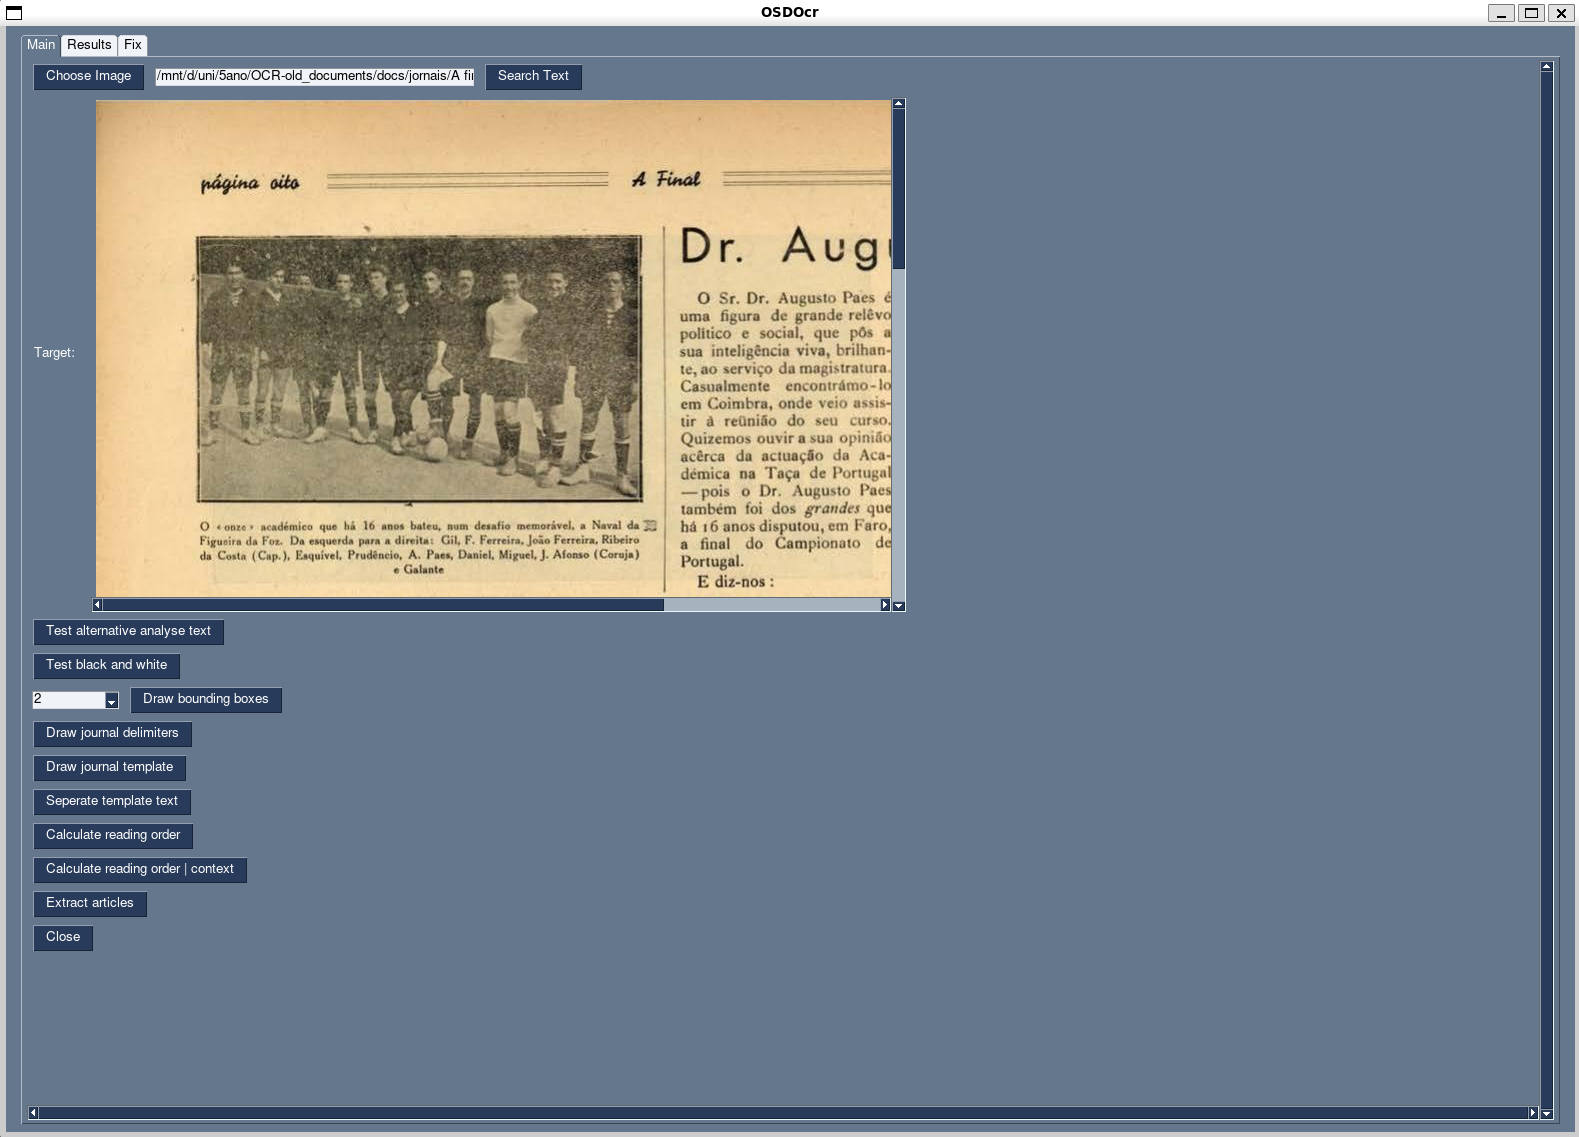
\includegraphics[width=1\textwidth]{images/implementacao/gui/gui_base.png}
    \caption{Interface gráfica simples}
    \label{fig:gui_base}
\end{figure}

\subsubsection{Visualização de bounding boxes}

\begin{figure}[H]
    \centering
    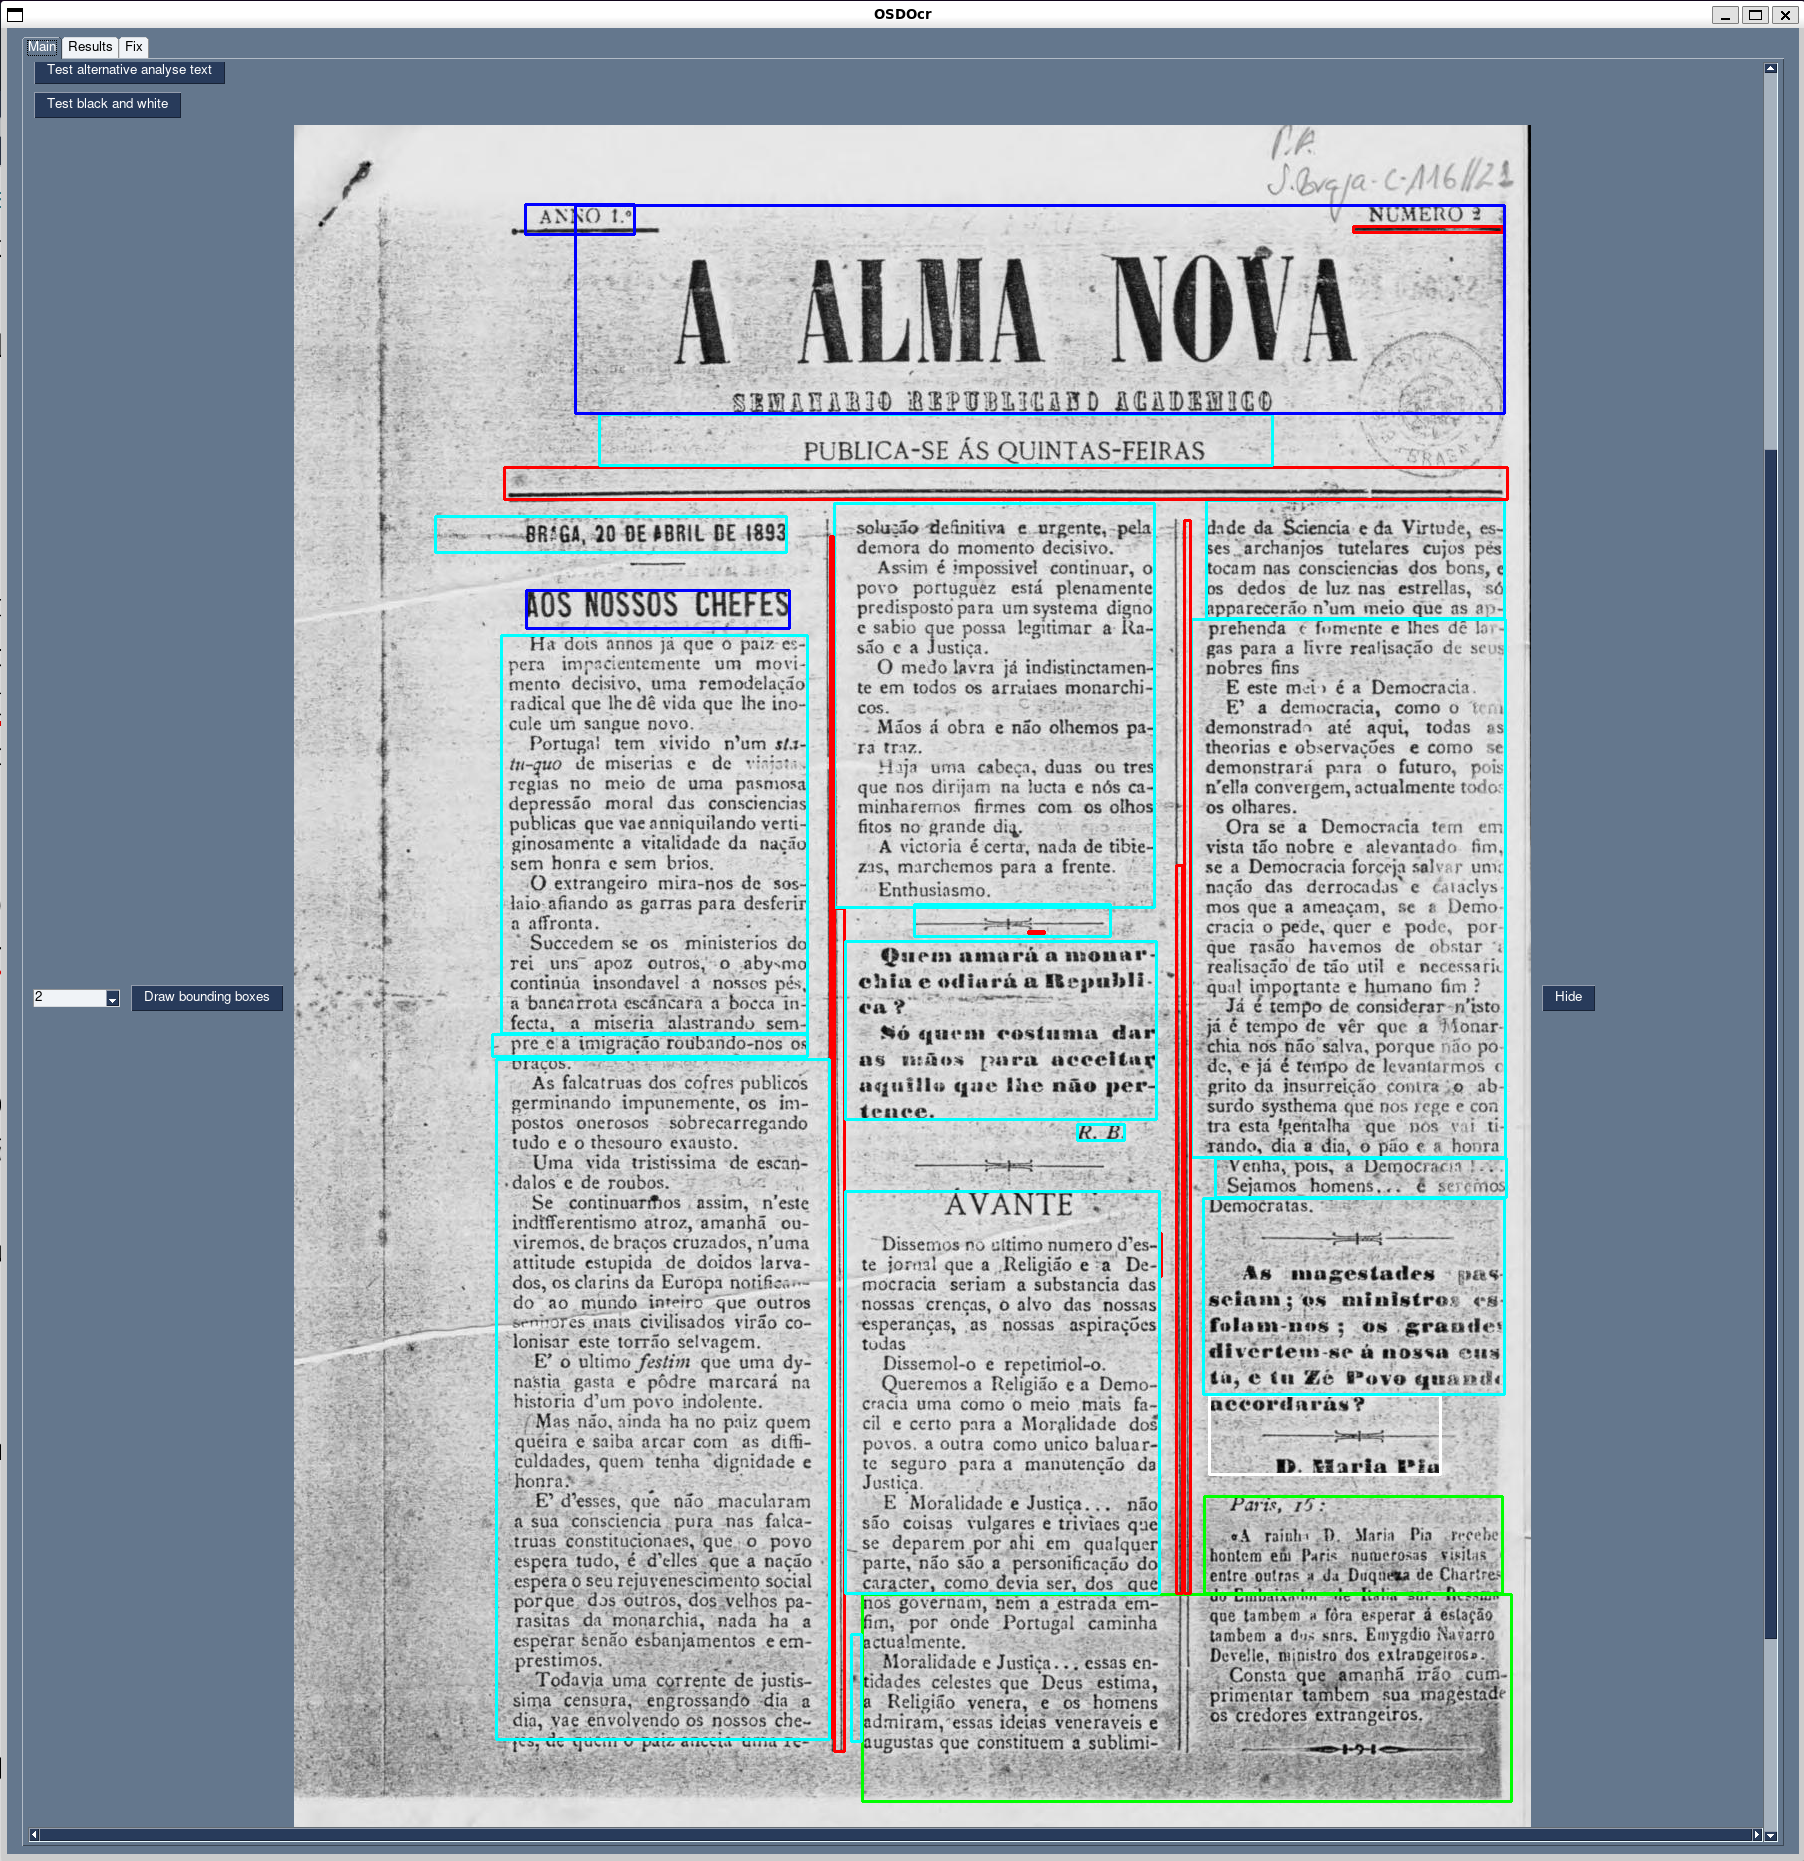
\includegraphics[width=1\textwidth]{images/implementacao/gui/gui_draw_bb.png}
    \caption{Visualização dos blocos resultantes de OCR}
    \label{fig:gui_draw_bb}
\end{figure}

A visualização de blocos dispõe também de coloração diferente para os blocos de acordo com a sua categorização. Blocos título estão a azul escuro, texto a azul claro, delimitadores a vermelho, legendas a branco e o resto - imagens, outros - a verde.

\subsubsection{Cálculo de template de jornal}

\begin{figure}[H]
    \centering
    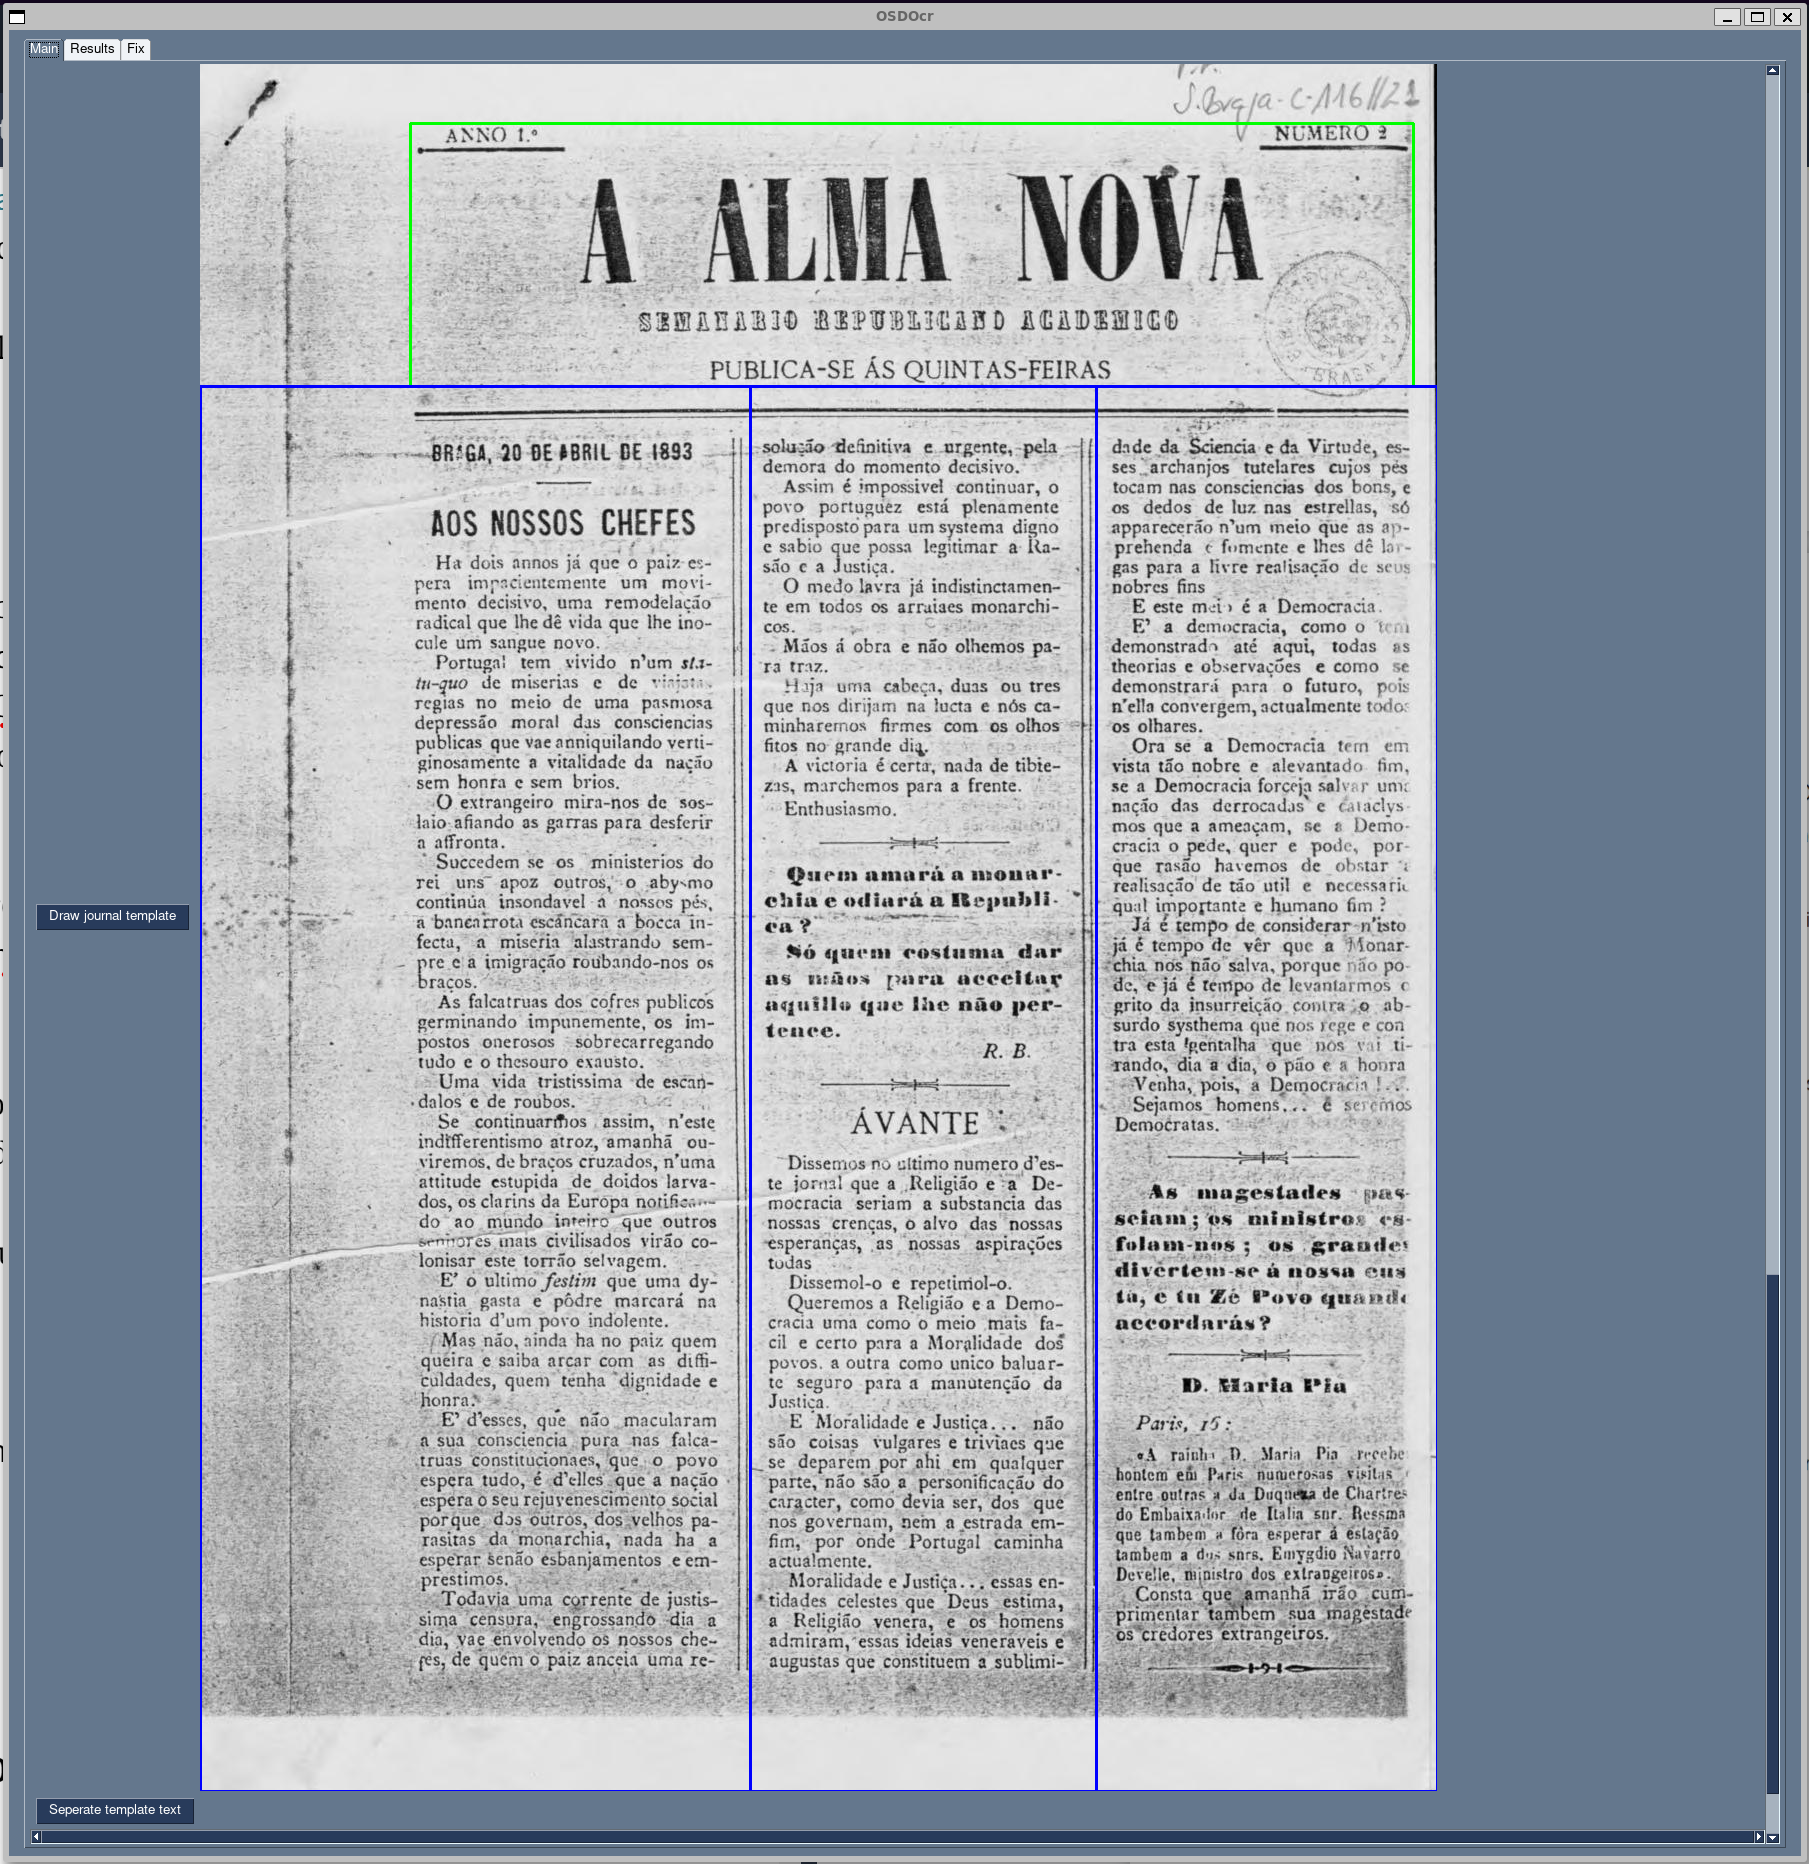
\includegraphics[width=1\textwidth]{images/implementacao/gui/gui_draw_template.png}
    \caption{Visualização do cálculo do template de jornal}
    \label{fig:gui_draw_template}
\end{figure}

O cálculo de template é feito através da deteção e análise dos delimitadores dos resultados OCR. Áreas são depois calculadas de acordo com estes delimitadores e, como se pode ver no caso do Header (caixa a verde) da imagem \ref{fig:gui_draw_template}, a área é ajustada de acordo com as caixas com texto da respetiva área.

\subsubsection{Extração de artigos}

\begin{figure}[H]
    \centering
    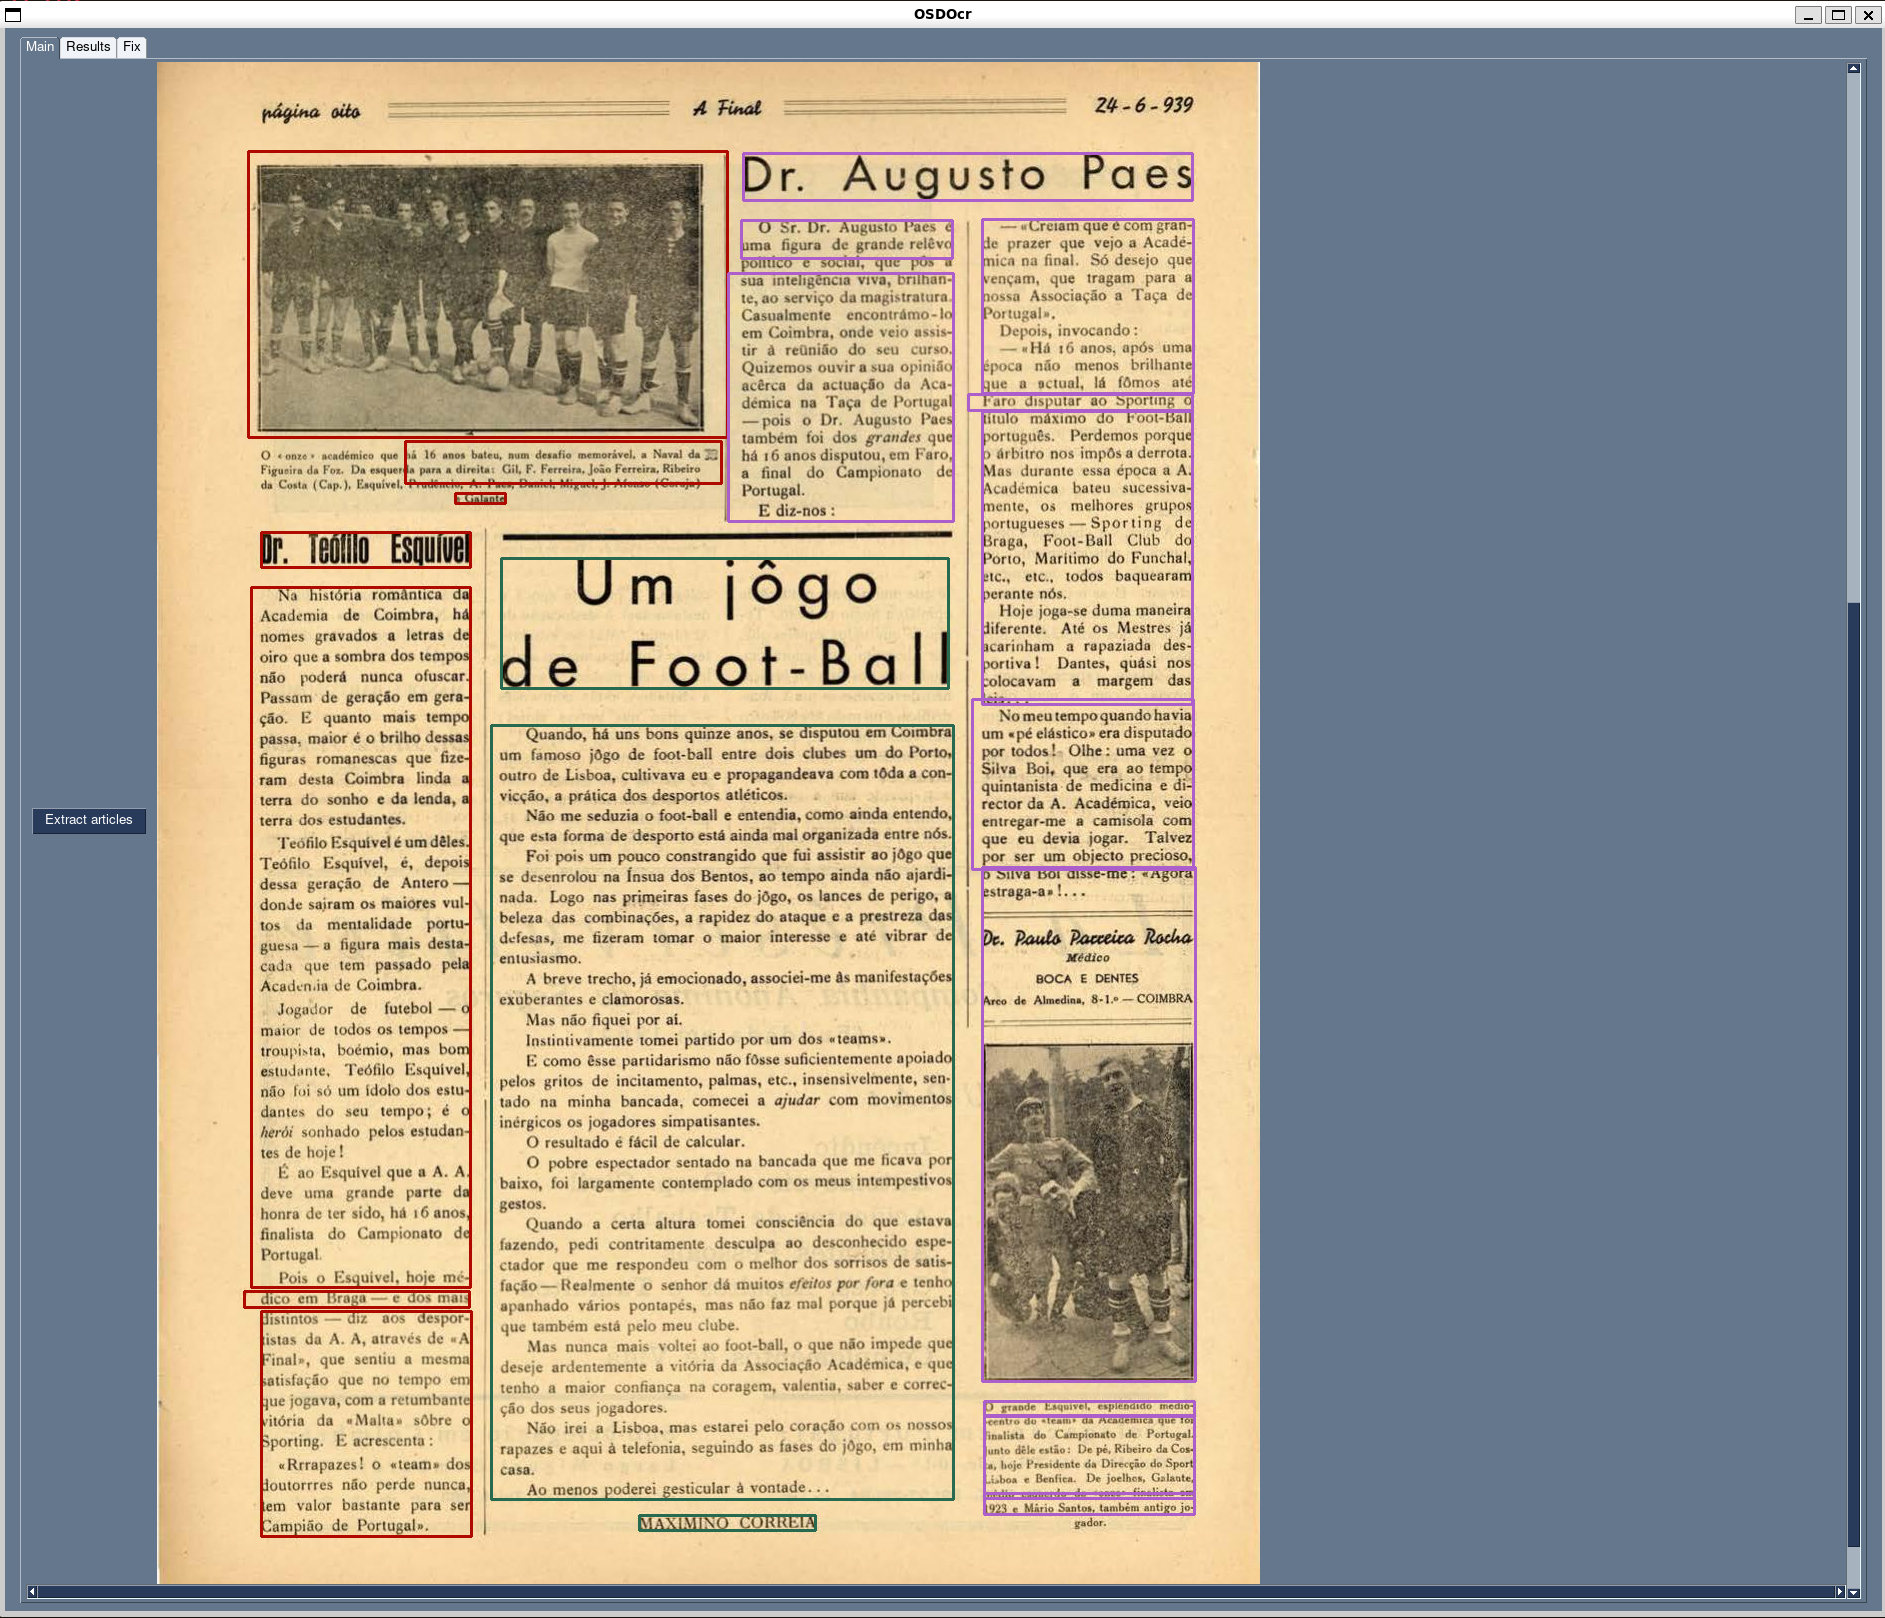
\includegraphics[width=1\textwidth]{images/implementacao/gui/gui_draw_articles.png}
    \caption{Visualização dos artigos extraídos}
    \label{fig:gui_draw_article}
\end{figure}

Neste caso, os artigos são calculados e posteriormente escolhidas cores distintas para realçar cada um destes. Os artigos são representados pelo conjunto de blocos que foram agrupados como sendo um dado artigo.

\subsubsection{Limpeza de bounding boxes}

\begin{figure}[H]
    \centering
    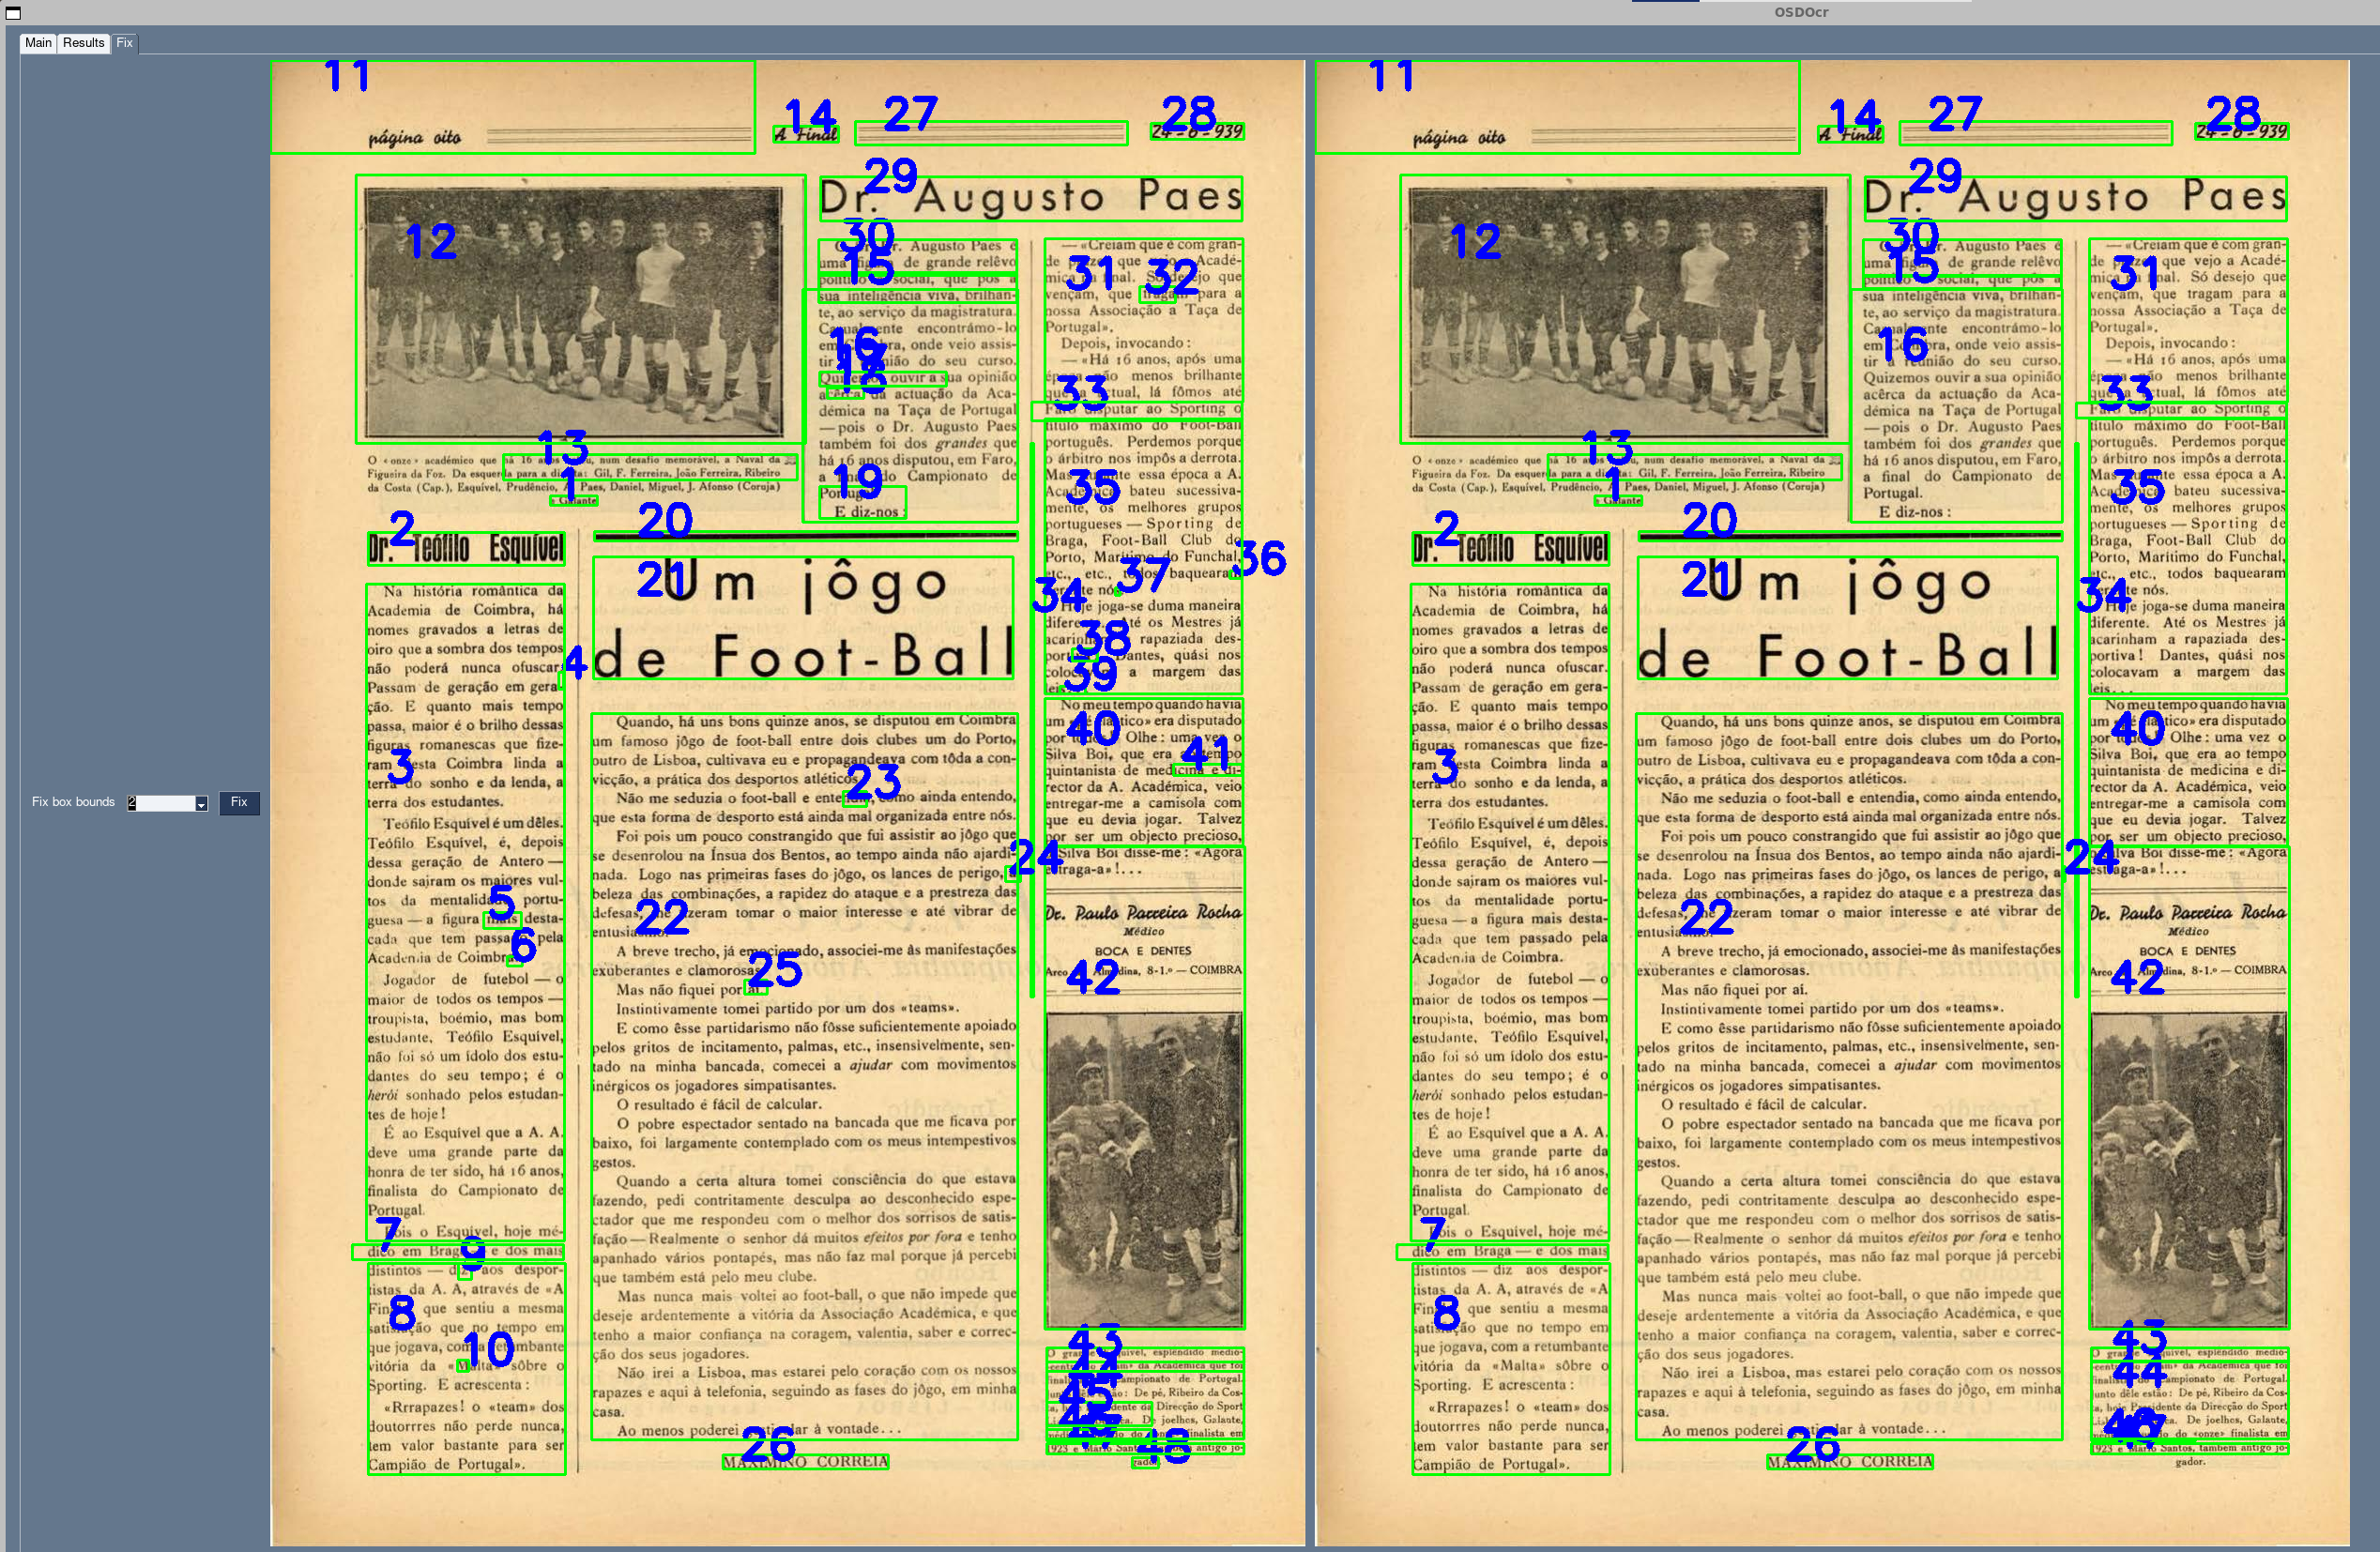
\includegraphics[width=1\textwidth]{images/implementacao/gui/gui_fix_blocks.png}
    \caption{Visualização da limpeza de blocos}
    \label{fig:gui_fix_bb}
\end{figure}

Para facilitar a deteção das diferenças entre o antes e depois da limpeza, os dois estados são postos lado a lado e os blocos são identificados, mantendo a mesma identificação após a limpeza. 




\section{Categorização de blocos}
\label{categorizacao_blocos}

Como verificado em vários dos estudos no estado da arte, por vezes, para realizar a segmentação correta dos documentos, é necessário considerar mais do que as posições relativas entre as diferentes caixas de texto. Por isto, um categorização destas caixas através de uma análise das suas características, permite o armazenamento de algum contexto sobre estas.

Atualmente, as caixas são categorizados em 1 destes tipos:

\begin{itemize}
    \item \textbf{Delimitador} : Caixa vazia (sem texto) e que cumpre a regra:

        $box.width >= 4*box.height \vee box.height >= 4*box.width$
        \item \textbf{Texto} : Tamanho médio do texto é do tamanho médio do documento, com uma margem de 30\%. Necessita uma análise de texto do documento.
        \item  \textbf{Título} : Tamanho médio acima do tamanho médio do documento.
        \item \textbf{Legenda} : Tamanho médio abaixo do tamanho médio do documento.
        \item \textbf{Outro} : Para as caixas que não correspondem a nenhum dos outros casos. Método provisório para categorizar imagens e outros elementos sem texto.
\end{itemize}

    Além disso, para as caixas com texto, verificam-se algumas características deste, nomeadamente:
    \begin{itemize}
        \item \textbf{Texto iniciado} : Se a primeira letra for maiúscula.
        \item \textbf{Texto não terminado} : Se não tiver terminado com uma pontuação de fim de frase.
    \end{itemize}

A figura \ref{fig:gui_draw_bb} apresenta os blocos categorizados através deste algoritmo.

Trabalho futuro neste procedimento, consistirá em, além das melhorias na categorização já realizada, possibilitar a identificação de outras entidades como imagens, anúncios ou tabelas.

\section{Limpeza de blocos}
\label{limpeza_blocos}

Como se pode observar na imagem da esquerda da figura \ref{fig:gui_fix_bb}, os resultados de OCR podem vir com bastantes defeitos, tais como: caixas sobrepostas, caixas intersetadas, caixas que capturam sujidade ou ruído.

Tal dificulta a análise e em especial a segmentação do documento. Deste modo, é essencial um processo de pós processamento para limpeza dos blocos e, assim, reduzir a quantidade de informação a trabalhar.

Neste momento, o algoritmo desenvolvido procura remover caixas vazias, inclusive as sobrepostas e remover interseções de caixas. Um traço geral está descrito em baixo.

\begin{algorithm}[H]
    \caption{Limpeza de blocos}
    \begin{algorithmic}[1]
    
    \STATE analyze\_text()

    \WHILE{Não verificou todos os blocos}
        \STATE Escolher próximo bloco a analisar 
        \COMMENT{Não pode ser vazio, a não ser que seja delimitador}

        \IF{Bloco a analisar está dentro do próximo bloco, ou vice-versa}
            \IF{Próximo bloco é vazio, não delimitador}
                \STATE remove\_block()
            \ENDIF
        \ENDIF

        \IF{Bloco a analisar e próximo bloco intersetam-se}
            \STATE remove\_box\_area(intersection\_area)
        \ENDIF

        \STATE Adicionar bloco a analisar como verificado
    \ENDWHILE

    \RETURN Blocos limpos
    
\end{algorithmic}
\end{algorithm}

No exemplo da figura \ref{fig:gui_fix_bb} o número de blocos foi reduzido de 49 para 30.

Alguns aspetos que têm de ser melhorados são: reduzir dimensões dos blocos para assemelhar ao texto que engloba; no tratamento de interseções, tratar o texto que estiver na área modificada.


\section{Análise de texto}
\label{analise_texto}

A análise de texto permite acrescentar características aos blocos além das suas posições geométricas. Como já referido na secção \ref{categorizacao_blocos}, o simples cálculo do tamanho normal do texto permite criar uma métrica relativamente confiável para distinguir, por exemplo, títulos de texto normal. Atualmente, o algoritmo implementado apenas calcula algumas métricas simples:
\begin{itemize}
    \item Tamanho de texto normal
    \item Espaçamento médio do texto
    \item Número de colunas provável (através da análise das margens comuns do texto)
\end{itemize}

\begin{algorithm}[H]
    \caption{Análise de texto}
    \begin{algorithmic}[1]

    \FOR{linhas}
        \STATE Guardar tamanho médio de linha
        \STATE Guardar margens da linha
    \ENDFOR

    \STATE normal\_text\_size $\gets$ média do tamanho das linhas
    \STATE desvio\_padrao $\gets$ calculo desvio padrao do tamanho das linhas
    \WHILE{$\text{normal\_text\_size\_std} > \text{normal\_text\_size} \times 2$}
        \STATE remover outlier
        \STATE recalcular normal\_text\_size e desvio\_padrao
    \ENDWHILE

    \STATE calcular margens esquerdas mais comuns
    \STATE estimar número de colunas de acordo com margens esquerdas
    
\end{algorithmic}
\end{algorithm}

No futuro, outras estatísticas deverão ser acrescentadas, assim como o aperfeiçoamento do cálculo das presentes.


\section{Ordenação de blocos}
\label{ordenacao_blocos}

Como observado no estado da arte, documentos complexos, como são exemplo jornais, necessitam um maior cuidado na reconstrução do seu conteúdo em comparação com documentos mais simples como um livro regular. Isto deve-se ao facto dos elementos de texto que o compõe nem sempre seguem uma ordem simples (cima para baixo e esquerda para a direita), sendo muitas vezes irregulares e dependentes de alguma forma de contexto, seja delimitadores, imagens ou mesmo o conteúdo do texto.

Deste modo, o cálculo da ordem de leitura dos resultados de OCR é uma das tarefas primárias deste projeto.

Atualmente, a implementação da ordenação de blocos, segue métodos de heurísticas utilizando grafos. Tal permite, como em casos observados em trabalhos relacionados na secção  \ref{sec_trab_relacionado}, a combinação de ordenação tendo em conta a posição dos blocos e também, pelo peso entre os nodos, correspondente a um nível de atração calculado tendo em conta o contexto.

Assumindo um pós processamento de limpeza dos blocos, começa-se com a criação de um grafo de ligação entre os blocos. As ligações criadas entre os blocos neste ponto seguem apenas regras simples de posição relativa, i.e. um bloco apenas pode ter como filhos blocos, adjacentes, por baixo de si ou diretamente à sua direita.

Com o grafo criado, segue-se o cálculo dos pesos. Estes tomam em conta tanto a posição relativa dos blocos, sendo que por norma um bloco tem tendência a ser seguido por um bloco abaixo, mas também o contexto, permitindo corrigir este preconceito quando evidente. O contexto atualmente considerado é:
\begin{itemize}
    \item \textbf{Categoria dos blocos} : certos tipos de blocos são mais atraídos por tipos específicos. Ex.: imagem e legenda; título e bloco não título.
    \item \textbf{Características de blocos de texto} : caso um bloco de texto não esteja acabado, então ele é naturalmente mais atraído para blocos de texto que não estejam iniciados.
\end{itemize}

Procede-se com uma poda das ligações de filhos para pais de forma a remover ligações com atração muito baixa e assim reduzir dependências dos nodos. A remoção é realizada quando entre dois nodos existem ligações que tenham peso duas ou mais vezes maior do que as outras.

Por último, o grafo é ordenado pelo caminho de maior custo. Tem-se aqui em conta que o próximo nodo escolhido para ordenar não pode ter dependências ativas, i.e. todos os seus potenciais pais têm de já ter sido escolhidos.

\begin{figure}[H]
    \hspace*{-4.5cm}
    \includegraphics[width=1.5\textwidth]{images/implementacao/algoritmos/comparacao_ordem_leitura.png}
    \caption{Comparação de ordens de leitura: (a) ordem correta; (b) ordem do Tesseract; (c) ordem do algoritmo implementado}
    \label{fig:comp_reading_order}
\end{figure}

Como se observa na imagem \ref{fig:comp_reading_order}, para o exemplo desta página de jornal, a ordem de leitura calculada pelo algoritmo, embora com alguns erros, assemelha-se significativamente mais À correta do que a fornecida pelo Tesseract.



Esta implementação ainda pode ser denotada como \textit{naive} visto ainda incluir pouco contexto na sua lógica. Outras implementações terão de ser experimentadas e comparadas no futuro.

No entanto, este ponto de partida já permite uma extração simples de artigos. Tendo em conta a ordem de leitura e, assumindo que um artigo é sempre inicializado por um título, podemos cortar a sequência ordenada das caixas pelos seus títulos e assim dividir em artigos. A figura \ref{fig:gui_draw_article} é um exemplo disto. É de notar no entanto, que uma posterior ordenação destes artigos poderia ser realizada.
